
\subsubsection{\stid{2.08} HPCToolkit} 
\paragraph{Overview} 

The HPCToolkit project is working to develop performance measurement
and analysis tools to help ECP application, library, runtime, and tool
developers understand where and why their software does not fully
exploit hardware resources within and across nodes of extreme-scale
parallel systems. Key deliverables of the project are a suite of
software tools that developers need to measure and analyze the
performance of parallel software as it executes on existing ECP
testbeds and new technologies needed to measure and analyze
performance on forthcoming exascale systems.

To provide a foundation for performance measurement and analysis, the
project team is working with community stakeholders, including
standards committees, vendors, and open source developers to improve
hardware and software support for measurement and attribution of
application performance on extreme-scale parallel systems. The
project team has been engaging vendors to improve hardware support
for performance measurement in next generation systems and working
with other software teams to design and integrate new capabilities
into operating systems, runtime systems, communication libraries, and
application frameworks that will enhance the ability of software
tools to accurately measure and attribute code performance on
extreme-scale parallel systems.  Using emerging hardware and software
interfaces for monitoring code performance, the project team is
working to extend capabilities to measure computation, data movement,
communication, and I/O as a program executes to pinpoint scalability
bottlenecks, quantify resource consumption, and assess
inefficiencies.

\paragraph{Key  Challenges}

In recent years, the complexity, diversity, and the rate of change of
architectures for extreme-scale parallel systems have increased
dramatically. For higher efficiency, heterogeneous designs that couple
multicore processors with accelerators and employ more complex memory
hierarchies are now common. In addition, the DOE is purposefully
pursuing multiple independent architectural designs for next
generation parallel systems as part of risk mitigation. For
performance tools, the need to support multiple diverse architectural
paths significantly increases tool complexity.  At the same time, the
complexity of applications is increasing dramatically as developers
struggle to expose billion-way parallelism, map computation onto
heterogeneous computing elements, and cope with the growing complexity
of memory hierarchies. While application developers can employ
abstractions to hide some of the complexity of emerging parallel
systems, performance tools must be intimately familiar with each of
the features added to these systems to improve performance or
efficiency, develop measurement and analysis techniques that assess
how well these features are being exploited, and then relate these
measurements back to software to create actionable feedback that will
guide developers to improve the performance, efficiency, and
scalability of their applications.

\paragraph{Solution Strategy}

Development of HPCToolkit as part of ECP is focused on preparing it
for production use at exascale by enhancing it in several ways. First,
the team is adding new capabilities to measure and analyze
interactions between software and key hardware subsystems in
extreme-scale platforms, including more complex memory hierarchies and
accelerators. Second, the team is working to improve performance
attribution given optimized code for complex node-level programming
models used by ECP developers, including OpenMP and template-based
programming models such as LLNL's RAJA and Sandia's KOKKOS. To support
this effort, the project team is enhancing the Dyninst binary analysis
toolkit, which is also used by other ECP tools. Third, the team is
improving the scalability of HPCToolkit so that it can be used to
measure and analyze extreme-scale executions. Fourth, the project team
is working to improve the robustness of the tools across the range of
architectures used as ECP platforms. Finally, the project team will
work other ECP teams to ensure that they benefit from HPCToolkit's
capabilities to measure, analyze, attribute, and diagnose performance
issues on ECP testbeds and forthcoming exascale systems.

\paragraph{Recent Progress}

\begin{itemize}

\item
The project team developed novel capabilities for attributing
performance metrics to accelerated applications that offload
computation onto NVIDIA GPUs.  To support hierarchical attribution of
GPU performance metrics gathered using PC sampling, HPCToolkit
reconstructs the program structure for GPU machine code, including
static call chains and loop nests.
% HPCToolkit recovers control flow graphs for GPU procedures, analyzes
% their structure to identify loops, reconstructs static call chains
% by analyzing procedure calls in GPU machine code, maps GPU machine
% code to source lines and inlined procedures, and approximately
% apportions costs among call sites to a GPU function by using PC
% samples for call instructions as a guide.
Figure~\ref{fig:hpctoolkit}(a) illustrates how HPCToolkit attributes
contexts to GPU computations specified using OpenMP TARGET constructs.

\item
The project team developed novel capabilities for profiling and
tracing applications that dynamically create many short-lived
threads. Figure~\ref{fig:hpctoolkit}(b) shows a trace of a
quantum materials code where multiple short-lived threads with
non-overlapping lifetimes are fused into compact timelines.

 \item 
To accelerate analysis necessary to attribute execution
performance to large application binaries, the project team developed
a new version of HPCToolkit's hpcstruct utility that employs OpenMP
tasks to parse and analyze machine code for application functions in
parallel. Parallel parsing of machine code was released in November
2018 as part of Dyninst 10.0.

\item
The project PI successfully led the development of OMPT --- a
first-party tools API for OpenMP. The OMPT API was released as part of
the OpenMP 5.0 standard in November 2018.

\item 
The project team developed a Spack release of HPCToolkit with all of
HPCToolkit's dependencies fully exposed.

\end{itemize}

\begin{figure}[t]
\captionsetup{width=.96\textwidth}
\begin{minipage}[t]{.48\textwidth}
\centering
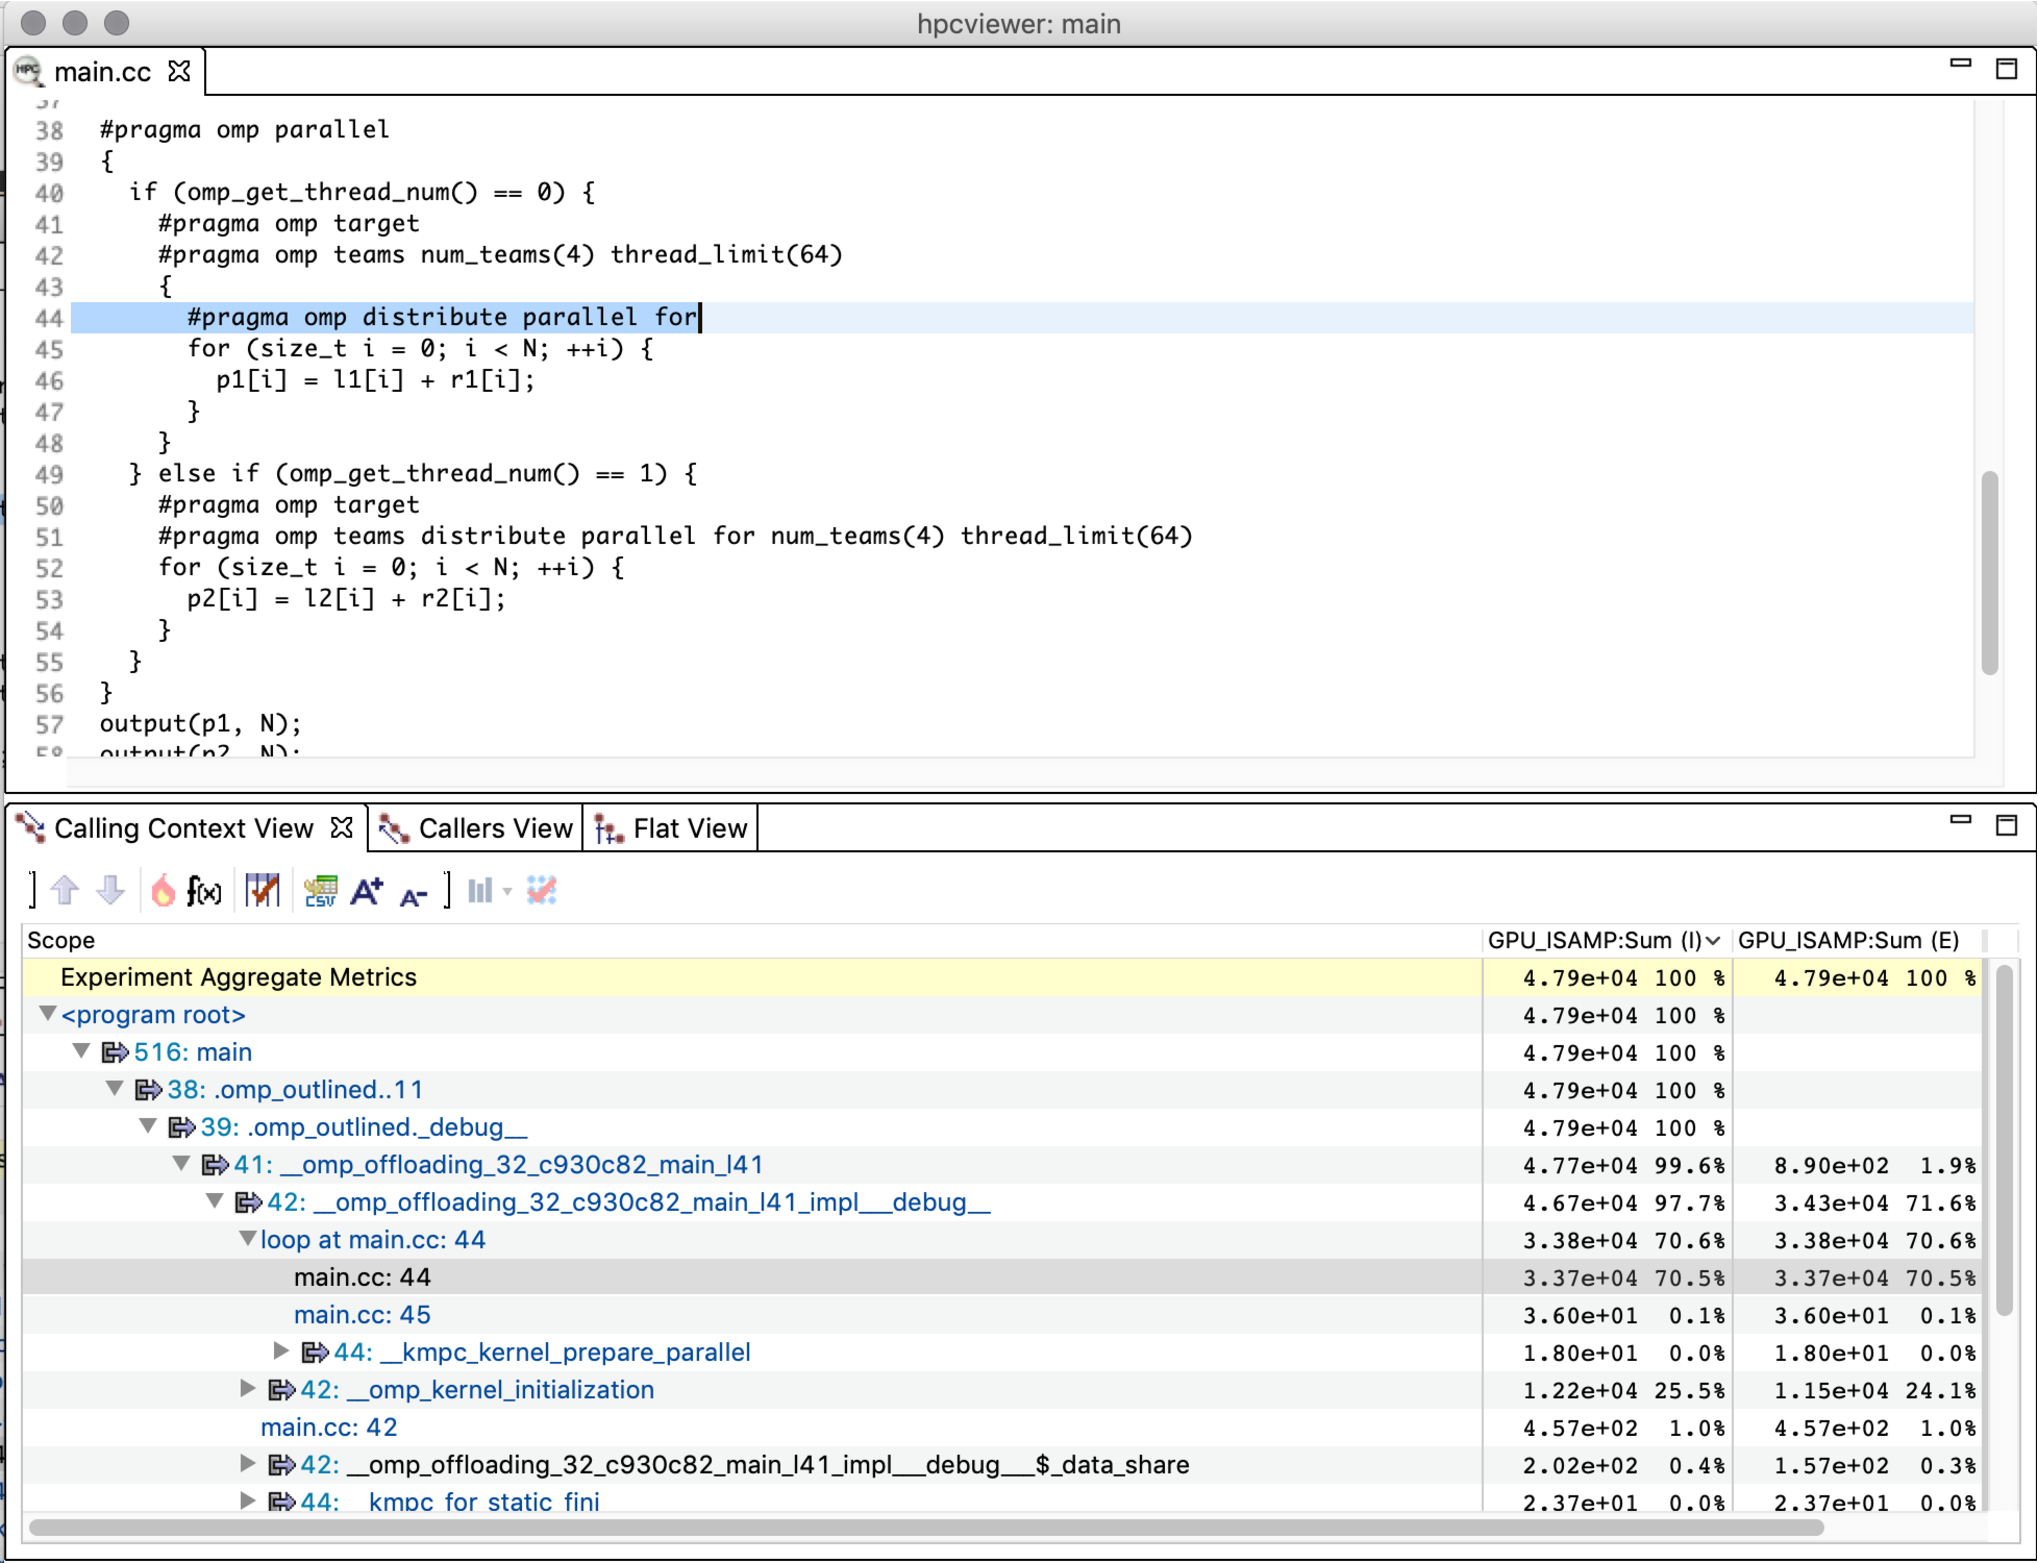
\includegraphics[width=\textwidth]{projects/2.3.2-Tools/2.3.2.08-HPCToolkit/hpctoolkit-vec-add-ompt}
\\(a)
\end{minipage}
\hfill
\begin{minipage}[t]{.48\textwidth}
\centering
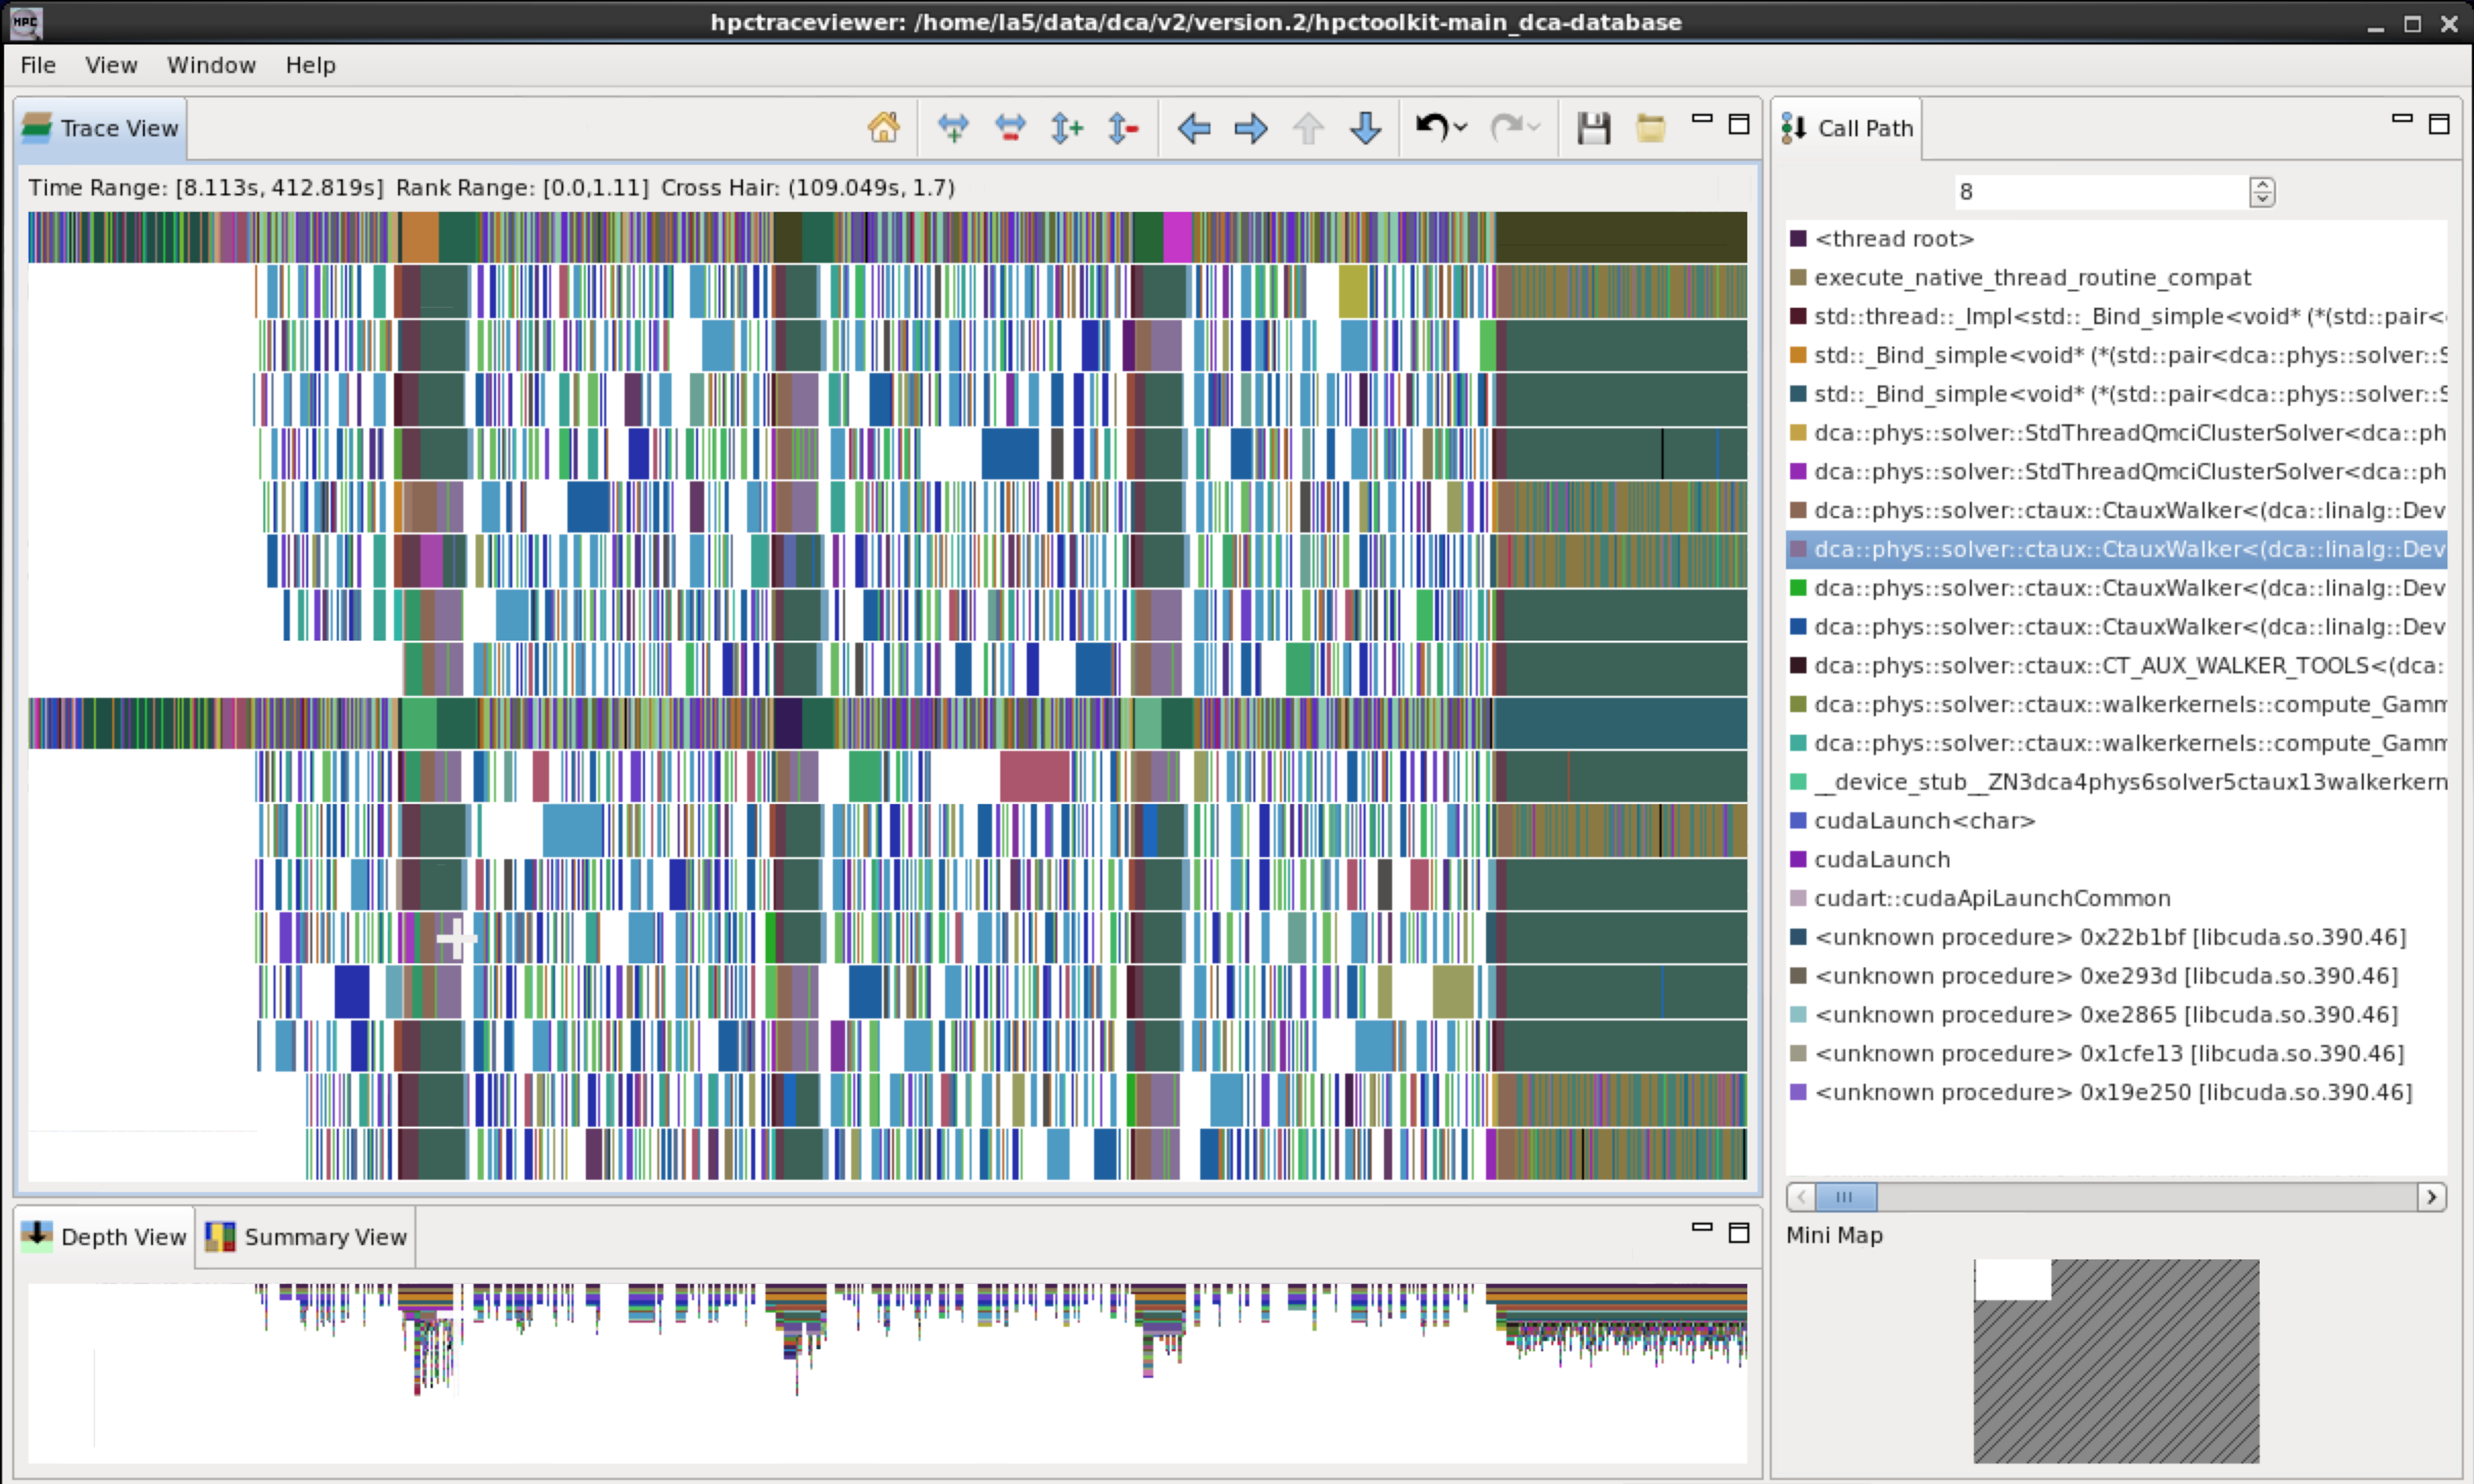
\includegraphics[width=\textwidth]{projects/2.3.2-Tools/2.3.2.08-HPCToolkit/hpctoolkit-many-threads}
\\(b)
\end{minipage}
\caption{(a) 
HPCToolkit's {\tt hpcviewer} showing a detailed attribution of GPU performance metrics in a 
profile of an optimized, GPU-accelerated benchmark written in 
OpenMP~5.0.
(b) HPCToolkit's {\tt hpctraceviewer} showing an execution trace of DCA+ --- a quantum Monte Carlo code that
creates many short-lived threads as it simulates correlated electron
systems in high temperature superconductors.}
\label{fig:hpctoolkit}
\end{figure}

\paragraph{Next Steps}
\begin{itemize}

\item 
Refine new capabilities and integrate them into HPCToolkit's trunk for
release.

\item 
Refine the Spack configuration for HPCToolkit to exploit
vendor-provided MPI and manage differences between host and compute
nodes.

\item 
Work with open source community to upstream GPU measurement support
developed by the project team into the community version of the {\tt
libomptarget} offloading library.

\item 
Complete new measurement capabilities that leverage the new
first-party tools API in OpenMP 5.0 to asynchronously reconstruct
user-level calling contexts for nested parallel regions and tasks at
runtime.

\item 
Complete work on data-centric performance analysis capabilities that
measure and attribute data movement costs to program variables.

\item 
Work with DOE and platform vendors to co-design performance
measurement technologies for forthcoming exascale platforms, including
A21.

\end{itemize}
